\documentclass[twoside]{book}

% Packages required by doxygen
\usepackage{fixltx2e}
\usepackage{calc}
\usepackage{doxygen}
\usepackage[export]{adjustbox} % also loads graphicx
\usepackage{graphicx}
\usepackage[utf8]{inputenc}
\usepackage{makeidx}
\usepackage{multicol}
\usepackage{multirow}
\PassOptionsToPackage{warn}{textcomp}
\usepackage{textcomp}
\usepackage[nointegrals]{wasysym}
\usepackage[table]{xcolor}

% Font selection
\usepackage[T1]{fontenc}
\usepackage[scaled=.90]{helvet}
\usepackage{courier}
\usepackage{amssymb}
\usepackage{sectsty}
\renewcommand{\familydefault}{\sfdefault}
\allsectionsfont{%
  \fontseries{bc}\selectfont%
  \color{darkgray}%
}
\renewcommand{\DoxyLabelFont}{%
  \fontseries{bc}\selectfont%
  \color{darkgray}%
}
\newcommand{\+}{\discretionary{\mbox{\scriptsize$\hookleftarrow$}}{}{}}

% Page & text layout
\usepackage{geometry}
\geometry{%
  a4paper,%
  top=2.5cm,%
  bottom=2.5cm,%
  left=2.5cm,%
  right=2.5cm%
}
\tolerance=750
\hfuzz=15pt
\hbadness=750
\setlength{\emergencystretch}{15pt}
\setlength{\parindent}{0cm}
\setlength{\parskip}{3ex plus 2ex minus 2ex}
\makeatletter
\renewcommand{\paragraph}{%
  \@startsection{paragraph}{4}{0ex}{-1.0ex}{1.0ex}{%
    \normalfont\normalsize\bfseries\SS@parafont%
  }%
}
\renewcommand{\subparagraph}{%
  \@startsection{subparagraph}{5}{0ex}{-1.0ex}{1.0ex}{%
    \normalfont\normalsize\bfseries\SS@subparafont%
  }%
}
\makeatother

% Headers & footers
\usepackage{fancyhdr}
\pagestyle{fancyplain}
\fancyhead[LE]{\fancyplain{}{\bfseries\thepage}}
\fancyhead[CE]{\fancyplain{}{}}
\fancyhead[RE]{\fancyplain{}{\bfseries\leftmark}}
\fancyhead[LO]{\fancyplain{}{\bfseries\rightmark}}
\fancyhead[CO]{\fancyplain{}{}}
\fancyhead[RO]{\fancyplain{}{\bfseries\thepage}}
\fancyfoot[LE]{\fancyplain{}{}}
\fancyfoot[CE]{\fancyplain{}{}}
\fancyfoot[RE]{\fancyplain{}{\bfseries\scriptsize Generated by Doxygen }}
\fancyfoot[LO]{\fancyplain{}{\bfseries\scriptsize Generated by Doxygen }}
\fancyfoot[CO]{\fancyplain{}{}}
\fancyfoot[RO]{\fancyplain{}{}}
\renewcommand{\footrulewidth}{0.4pt}
\renewcommand{\chaptermark}[1]{%
  \markboth{#1}{}%
}
\renewcommand{\sectionmark}[1]{%
  \markright{\thesection\ #1}%
}

% Indices & bibliography
\usepackage{natbib}
\usepackage[titles]{tocloft}
\setcounter{tocdepth}{3}
\setcounter{secnumdepth}{5}
\makeindex

% Hyperlinks (required, but should be loaded last)
\usepackage{ifpdf}
\ifpdf
  \usepackage[pdftex,pagebackref=true]{hyperref}
\else
  \usepackage[ps2pdf,pagebackref=true]{hyperref}
\fi
\hypersetup{%
  colorlinks=true,%
  linkcolor=blue,%
  citecolor=blue,%
  unicode%
}

% Custom commands
\newcommand{\clearemptydoublepage}{%
  \newpage{\pagestyle{empty}\cleardoublepage}%
}

\usepackage{caption}
\captionsetup{labelsep=space,justification=centering,font={bf},singlelinecheck=off,skip=4pt,position=top}

%===== C O N T E N T S =====

\begin{document}

% Titlepage & ToC
\hypersetup{pageanchor=false,
             bookmarksnumbered=true,
             pdfencoding=unicode
            }
\pagenumbering{alph}
\begin{titlepage}
\vspace*{7cm}
\begin{center}%
{\Large My Project }\\
\vspace*{1cm}
{\large Generated by Doxygen 1.8.13}\\
\end{center}
\end{titlepage}
\clearemptydoublepage
\pagenumbering{roman}
\tableofcontents
\clearemptydoublepage
\pagenumbering{arabic}
\hypersetup{pageanchor=true}

%--- Begin generated contents ---
\chapter{Namespace Index}
\section{Namespace List}
Here is a list of all documented namespaces with brief descriptions\+:\begin{DoxyCompactList}
\item\contentsline{section}{\hyperlink{namespace_admin}{Admin} }{\pageref{namespace_admin}}{}
\item\contentsline{section}{\hyperlink{namespace_u_i}{UI} }{\pageref{namespace_u_i}}{}
\end{DoxyCompactList}

\chapter{Hierarchical Index}
\section{Class Hierarchy}
This inheritance list is sorted roughly, but not completely, alphabetically\+:\begin{DoxyCompactList}
\item \contentsline{section}{Account}{\pageref{class_account}}{}
\item \contentsline{section}{Admin}{\pageref{class_admin}}{}
\item \contentsline{section}{college}{\pageref{classcollege}}{}
\item \contentsline{section}{College}{\pageref{class_college}}{}
\item Q\+Main\+Window\begin{DoxyCompactList}
\item \contentsline{section}{admin\+Window}{\pageref{classadmin_window}}{}
\item \contentsline{section}{Create\+Login\+Window}{\pageref{class_create_login_window}}{}
\item \contentsline{section}{key\+Window}{\pageref{classkey_window}}{}
\item \contentsline{section}{login\+Window}{\pageref{classlogin_window}}{}
\item \contentsline{section}{Main\+Window}{\pageref{class_main_window}}{}
\item \contentsline{section}{shoppingcart}{\pageref{classshoppingcart}}{}
\end{DoxyCompactList}
\item Q\+Sql\+Database\begin{DoxyCompactList}
\item \contentsline{section}{Database}{\pageref{class_database}}{}
\end{DoxyCompactList}
\item Q\+Widget\begin{DoxyCompactList}
\item \contentsline{section}{Checkout\+Window}{\pageref{class_checkout_window}}{}
\end{DoxyCompactList}
\item \contentsline{section}{souvenir}{\pageref{classsouvenir}}{}
\item \contentsline{section}{Ui\+\_\+admin\+Window}{\pageref{class_ui__admin_window}}{}
\begin{DoxyCompactList}
\item \contentsline{section}{Ui\+:\+:admin\+Window}{\pageref{class_ui_1_1admin_window}}{}
\end{DoxyCompactList}
\item \contentsline{section}{Ui\+\_\+\+Checkout\+Window}{\pageref{class_ui___checkout_window}}{}
\begin{DoxyCompactList}
\item \contentsline{section}{Ui\+:\+:Checkout\+Window}{\pageref{class_ui_1_1_checkout_window}}{}
\end{DoxyCompactList}
\item \contentsline{section}{Ui\+\_\+\+Create\+Login\+Window}{\pageref{class_ui___create_login_window}}{}
\begin{DoxyCompactList}
\item \contentsline{section}{Ui\+:\+:Create\+Login\+Window}{\pageref{class_ui_1_1_create_login_window}}{}
\end{DoxyCompactList}
\item \contentsline{section}{Ui\+\_\+key\+Window}{\pageref{class_ui__key_window}}{}
\begin{DoxyCompactList}
\item \contentsline{section}{Ui\+:\+:key\+Window}{\pageref{class_ui_1_1key_window}}{}
\end{DoxyCompactList}
\item \contentsline{section}{Ui\+\_\+login\+Window}{\pageref{class_ui__login_window}}{}
\begin{DoxyCompactList}
\item \contentsline{section}{Ui\+:\+:login\+Window}{\pageref{class_ui_1_1login_window}}{}
\end{DoxyCompactList}
\item \contentsline{section}{Ui\+\_\+\+Main\+Window}{\pageref{class_ui___main_window}}{}
\begin{DoxyCompactList}
\item \contentsline{section}{Ui\+:\+:Main\+Window}{\pageref{class_ui_1_1_main_window}}{}
\end{DoxyCompactList}
\item \contentsline{section}{Ui\+\_\+shoppingcart}{\pageref{class_ui__shoppingcart}}{}
\begin{DoxyCompactList}
\item \contentsline{section}{Ui\+:\+:shoppingcart}{\pageref{class_ui_1_1shoppingcart}}{}
\end{DoxyCompactList}
\item \contentsline{section}{window\+Holder}{\pageref{classwindow_holder}}{}
\end{DoxyCompactList}

\chapter{Class Index}
\section{Class List}
Here are the classes, structs, unions and interfaces with brief descriptions\+:\begin{DoxyCompactList}
\item\contentsline{section}{\hyperlink{class_admin}{Admin} }{\pageref{class_admin}}{}
\item\contentsline{section}{\hyperlink{classadmin_window}{admin\+Window} }{\pageref{classadmin_window}}{}
\item\contentsline{section}{\hyperlink{classcollege}{college} }{\pageref{classcollege}}{}
\item\contentsline{section}{\hyperlink{class_college}{College} }{\pageref{class_college}}{}
\item\contentsline{section}{\hyperlink{class_create_login_window}{Create\+Login\+Window} }{\pageref{class_create_login_window}}{}
\item\contentsline{section}{\hyperlink{class_database}{Database} }{\pageref{class_database}}{}
\item\contentsline{section}{\hyperlink{classlogin_window}{login\+Window} }{\pageref{classlogin_window}}{}
\item\contentsline{section}{\hyperlink{class_ui_1_1_main_window}{Ui\+::\+Main\+Window} }{\pageref{class_ui_1_1_main_window}}{}
\item\contentsline{section}{\hyperlink{class_main_window}{Main\+Window} }{\pageref{class_main_window}}{}
\item\contentsline{section}{\hyperlink{class_q_main_window}{Q\+Main\+Window} }{\pageref{class_q_main_window}}{}
\item\contentsline{section}{\hyperlink{class_q_sql_database}{Q\+Sql\+Database} }{\pageref{class_q_sql_database}}{}
\item\contentsline{section}{\hyperlink{classsouvenir}{souvenir} }{\pageref{classsouvenir}}{}
\item\contentsline{section}{\hyperlink{class_the}{The} }{\pageref{class_the}}{}
\item\contentsline{section}{\hyperlink{class_ui___main_window}{Ui\+\_\+\+Main\+Window} }{\pageref{class_ui___main_window}}{}
\item\contentsline{section}{\hyperlink{classwindow_holder}{window\+Holder} }{\pageref{classwindow_holder}}{}
\end{DoxyCompactList}

\chapter{Namespace Documentation}
\hypertarget{namespace_admin}{}\section{Admin Namespace Reference}
\label{namespace_admin}\index{Admin@{Admin}}


\subsection{Detailed Description}
Window \hyperlink{namespace_u_i}{UI} 
\hypertarget{namespace_u_i}{}\section{UI Namespace Reference}
\label{namespace_u_i}\index{UI@{UI}}


\subsection{Detailed Description}
namespace for the Create Login Window Class
\chapter{Class Documentation}
\hypertarget{class_admin}{}\section{Admin Class Reference}
\label{class_admin}\index{Admin@{Admin}}


Collaboration diagram for Admin\+:\nopagebreak
\begin{figure}[H]
\begin{center}
\leavevmode
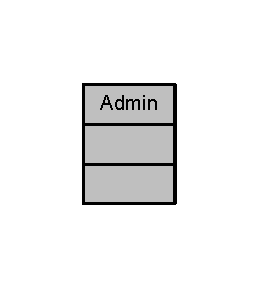
\includegraphics[width=124pt]{class_admin__coll__graph}
\end{center}
\end{figure}


The documentation for this class was generated from the following file\+:\begin{DoxyCompactItemize}
\item 
adminwindow.\+h\end{DoxyCompactItemize}

\hypertarget{classadmin_window}{}\section{admin\+Window Class Reference}
\label{classadmin_window}\index{admin\+Window@{admin\+Window}}


Inheritance diagram for admin\+Window\+:\nopagebreak
\begin{figure}[H]
\begin{center}
\leavevmode
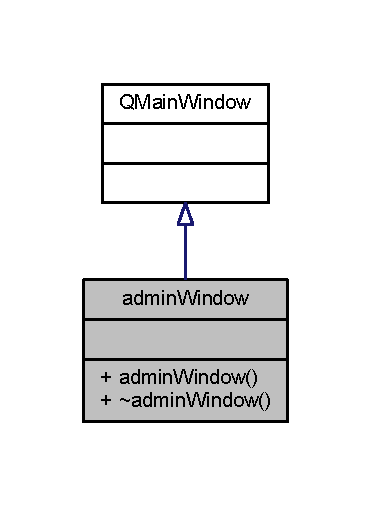
\includegraphics[width=160pt]{classadmin_window__inherit__graph}
\end{center}
\end{figure}


Collaboration diagram for admin\+Window\+:\nopagebreak
\begin{figure}[H]
\begin{center}
\leavevmode
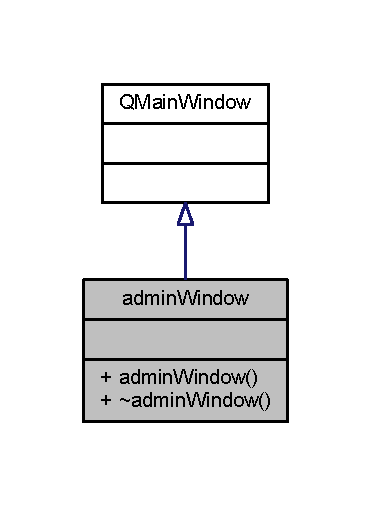
\includegraphics[width=160pt]{classadmin_window__coll__graph}
\end{center}
\end{figure}
\subsection*{Public Member Functions}
\begin{DoxyCompactItemize}
\item 
\hyperlink{classadmin_window_aa87a28958c1a314408df44e88c886ac5}{admin\+Window} (Q\+Widget $\ast$parent=0)
\item 
\mbox{\Hypertarget{classadmin_window_a95731b5313335ada974c1a4f2b7bc910}\label{classadmin_window_a95731b5313335ada974c1a4f2b7bc910}} 
void {\bfseries hide\+Group\+Boxes} ()
\item 
\mbox{\Hypertarget{classadmin_window_a83b7645ca3b45881681140f30d87d98a}\label{classadmin_window_a83b7645ca3b45881681140f30d87d98a}} 
void {\bfseries populate\+Add\+Souvenir\+CB} ()
\item 
\mbox{\Hypertarget{classadmin_window_a38fa5862c1ea91c2eb095339f7357078}\label{classadmin_window_a38fa5862c1ea91c2eb095339f7357078}} 
void {\bfseries populate\+School\+Name\+Delete\+DB} ()
\item 
\mbox{\Hypertarget{classadmin_window_aa2b416fe8b1d0848fc385102c1777a9c}\label{classadmin_window_aa2b416fe8b1d0848fc385102c1777a9c}} 
void {\bfseries populate\+School\+Name\+Modify\+CB} ()
\item 
\mbox{\Hypertarget{classadmin_window_a273e88bb1de74c5929fa58982fc527b0}\label{classadmin_window_a273e88bb1de74c5929fa58982fc527b0}} 
void {\bfseries populate\+Delete\+College\+CB} ()
\end{DoxyCompactItemize}


\subsection{Constructor \& Destructor Documentation}
\mbox{\Hypertarget{classadmin_window_aa87a28958c1a314408df44e88c886ac5}\label{classadmin_window_aa87a28958c1a314408df44e88c886ac5}} 
\index{admin\+Window@{admin\+Window}!admin\+Window@{admin\+Window}}
\index{admin\+Window@{admin\+Window}!admin\+Window@{admin\+Window}}
\subsubsection{\texorpdfstring{admin\+Window()}{adminWindow()}}
{\footnotesize\ttfamily admin\+Window\+::admin\+Window (\begin{DoxyParamCaption}\item[{Q\+Widget $\ast$}]{parent = {\ttfamily 0} }\end{DoxyParamCaption})\hspace{0.3cm}{\ttfamily [explicit]}}


\begin{DoxyParams}{Parameters}
{\em parent} & \\
\hline
\end{DoxyParams}


The documentation for this class was generated from the following files\+:\begin{DoxyCompactItemize}
\item 
adminwindow.\+h\item 
adminwindow.\+cpp\end{DoxyCompactItemize}

\hypertarget{classcollege}{}\section{college Class Reference}
\label{classcollege}\index{college@{college}}
\subsection*{Public Member Functions}
\begin{DoxyCompactItemize}
\item 
\hyperlink{classcollege_a14a1082be72591ff01ca864d92dd9887}{college} (Q\+String start, Q\+String end, bool boolean, double num)
\end{DoxyCompactItemize}
\subsection*{Public Attributes}
\begin{DoxyCompactItemize}
\item 
\mbox{\Hypertarget{classcollege_a91d5c57f0cbad290347af66575fd9df8}\label{classcollege_a91d5c57f0cbad290347af66575fd9df8}} 
Q\+String {\bfseries starting\+College}
\item 
\mbox{\Hypertarget{classcollege_a0aab2af26a9bc9a8a47b1e0040616ed1}\label{classcollege_a0aab2af26a9bc9a8a47b1e0040616ed1}} 
Q\+String {\bfseries ending\+College}
\item 
\mbox{\Hypertarget{classcollege_a0a46d7cad4b78170248ab1f5aa1649f0}\label{classcollege_a0a46d7cad4b78170248ab1f5aa1649f0}} 
bool {\bfseries visited}
\item 
\mbox{\Hypertarget{classcollege_a5b5ac9a4cd0c7dd201aaddb2cc5a6c27}\label{classcollege_a5b5ac9a4cd0c7dd201aaddb2cc5a6c27}} 
double {\bfseries distance}
\end{DoxyCompactItemize}


\subsection{Constructor \& Destructor Documentation}
\mbox{\Hypertarget{classcollege_a14a1082be72591ff01ca864d92dd9887}\label{classcollege_a14a1082be72591ff01ca864d92dd9887}} 
\index{college@{college}!college@{college}}
\index{college@{college}!college@{college}}
\subsubsection{\texorpdfstring{college()}{college()}}
{\footnotesize\ttfamily college\+::college (\begin{DoxyParamCaption}\item[{Q\+String}]{start,  }\item[{Q\+String}]{end,  }\item[{bool}]{boolean,  }\item[{double}]{num }\end{DoxyParamCaption})\hspace{0.3cm}{\ttfamily [inline]}}


\begin{DoxyItemize}
\item 
\begin{DoxyParams}{Parameters}
{\em start} & \\
\hline
\end{DoxyParams}

\item 
\begin{DoxyParams}{Parameters}
{\em end} & \\
\hline
\end{DoxyParams}

\item 
\begin{DoxyParams}{Parameters}
{\em boolean} & \\
\hline
\end{DoxyParams}

\item 
\begin{DoxyParams}{Parameters}
{\em int} & num \\
\hline
\end{DoxyParams}

\end{DoxyItemize}Assigns the starting college

Assigns the ending college

Assigns false to visited

Assigns the distance from starting college to ending college 

The documentation for this class was generated from the following file\+:\begin{DoxyCompactItemize}
\item 
collegestovisit.\+h\end{DoxyCompactItemize}

\hypertarget{class_college}{}\section{College Class Reference}
\label{class_college}\index{College@{College}}


Collaboration diagram for College\+:\nopagebreak
\begin{figure}[H]
\begin{center}
\leavevmode
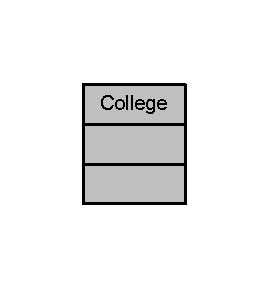
\includegraphics[width=129pt]{class_college__coll__graph}
\end{center}
\end{figure}


The documentation for this class was generated from the following file\+:\begin{DoxyCompactItemize}
\item 
collegestovisit.\+h\end{DoxyCompactItemize}

\hypertarget{class_create_login_window}{}\section{Create\+Login\+Window Class Reference}
\label{class_create_login_window}\index{Create\+Login\+Window@{Create\+Login\+Window}}


Inheritance diagram for Create\+Login\+Window\+:\nopagebreak
\begin{figure}[H]
\begin{center}
\leavevmode
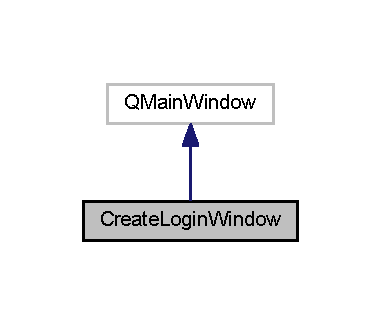
\includegraphics[width=183pt]{class_create_login_window__inherit__graph}
\end{center}
\end{figure}


Collaboration diagram for Create\+Login\+Window\+:\nopagebreak
\begin{figure}[H]
\begin{center}
\leavevmode
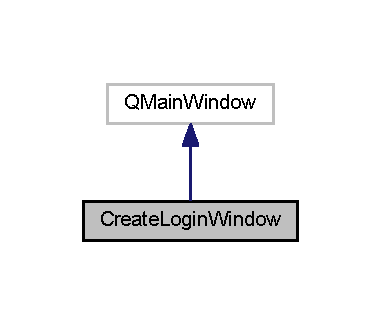
\includegraphics[width=183pt]{class_create_login_window__coll__graph}
\end{center}
\end{figure}
\subsection*{Public Member Functions}
\begin{DoxyCompactItemize}
\item 
\hyperlink{class_create_login_window_a5bddab7d05cb0e6b22dae4b96cc8ef13}{Create\+Login\+Window} (Q\+Widget $\ast$parent=0)
\end{DoxyCompactItemize}


\subsection{Detailed Description}

\begin{DoxyItemize}
\item 
\end{DoxyItemize}

\subsection{Constructor \& Destructor Documentation}
\mbox{\Hypertarget{class_create_login_window_a5bddab7d05cb0e6b22dae4b96cc8ef13}\label{class_create_login_window_a5bddab7d05cb0e6b22dae4b96cc8ef13}} 
\index{Create\+Login\+Window@{Create\+Login\+Window}!Create\+Login\+Window@{Create\+Login\+Window}}
\index{Create\+Login\+Window@{Create\+Login\+Window}!Create\+Login\+Window@{Create\+Login\+Window}}
\subsubsection{\texorpdfstring{Create\+Login\+Window()}{CreateLoginWindow()}}
{\footnotesize\ttfamily Create\+Login\+Window\+::\+Create\+Login\+Window (\begin{DoxyParamCaption}\item[{Q\+Widget $\ast$}]{parent = {\ttfamily 0} }\end{DoxyParamCaption})\hspace{0.3cm}{\ttfamily [explicit]}}


\begin{DoxyItemize}
\item 
\begin{DoxyParams}{Parameters}
{\em parent} & \\
\hline
{\em parent} & \\
\hline
\end{DoxyParams}

\end{DoxyItemize}

The documentation for this class was generated from the following files\+:\begin{DoxyCompactItemize}
\item 
createloginwindow.\+h\item 
createloginwindow.\+cpp\end{DoxyCompactItemize}

\hypertarget{class_database}{}\section{Database Class Reference}
\label{class_database}\index{Database@{Database}}


{\ttfamily \#include $<$database.\+h$>$}



Inheritance diagram for Database\+:\nopagebreak
\begin{figure}[H]
\begin{center}
\leavevmode
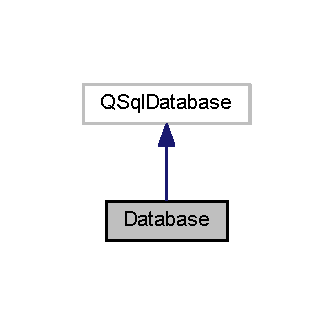
\includegraphics[width=160pt]{class_database__inherit__graph}
\end{center}
\end{figure}


Collaboration diagram for Database\+:\nopagebreak
\begin{figure}[H]
\begin{center}
\leavevmode
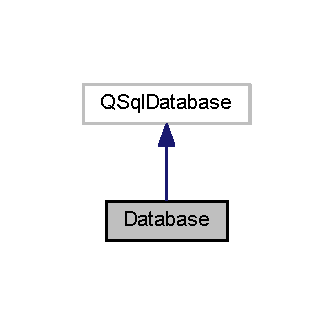
\includegraphics[width=160pt]{class_database__coll__graph}
\end{center}
\end{figure}
\subsection*{Public Member Functions}
\begin{DoxyCompactItemize}
\item 
\mbox{\Hypertarget{class_database_a76a9b0363174bdd6c70a052a088cfaf8}\label{class_database_a76a9b0363174bdd6c70a052a088cfaf8}} 
void {\bfseries add\+To\+Database} ()
\item 
\hyperlink{classcollege}{college} $\ast$ \hyperlink{class_database_affe7eb5c35db111e3ff7dc752f5a6c38}{get\+Closest\+School} (Q\+String school\+Name, Q\+Vector$<$ \hyperlink{classcollege}{college} $\ast$$>$ colleges\+To\+Visit)
\item 
int \hyperlink{class_database_aa5d167b5300b715844a760ed9d7e223f}{get\+Num\+Schools} ()
\end{DoxyCompactItemize}
\subsection*{Static Public Member Functions}
\begin{DoxyCompactItemize}
\item 
static \hyperlink{class_database}{Database} $\ast$ \hyperlink{class_database_a5a3b028f980a577ea0b809eb92312761}{get\+Instance} ()
\end{DoxyCompactItemize}


\subsection{Detailed Description}
Our database is a singleton because we dont want accidental copies 

\subsection{Member Function Documentation}
\mbox{\Hypertarget{class_database_affe7eb5c35db111e3ff7dc752f5a6c38}\label{class_database_affe7eb5c35db111e3ff7dc752f5a6c38}} 
\index{Database@{Database}!get\+Closest\+School@{get\+Closest\+School}}
\index{get\+Closest\+School@{get\+Closest\+School}!Database@{Database}}
\subsubsection{\texorpdfstring{get\+Closest\+School()}{getClosestSchool()}}
{\footnotesize\ttfamily \hyperlink{classcollege}{college} $\ast$ Database\+::get\+Closest\+School (\begin{DoxyParamCaption}\item[{Q\+String}]{school\+Name,  }\item[{Q\+Vector$<$ \hyperlink{classcollege}{college} $\ast$$>$}]{colleges\+To\+Visit }\end{DoxyParamCaption})}


\begin{DoxyItemize}
\item 
\begin{DoxyParams}{Parameters}
{\em school\+Name} & \\
\hline
\end{DoxyParams}

\item 
\begin{DoxyParams}{Parameters}
{\em colleges\+To\+Visit} & \\
\hline
\end{DoxyParams}

\item \begin{DoxyReturn}{Returns}

\end{DoxyReturn}
This function returns the name of the school thats closest and and the distance to it. It also does check to see if the school has already been visited to. 
\end{DoxyItemize}This loop finds the smallest distance from the school name passed in

prepares to find the index of the smallest distance \mbox{\Hypertarget{class_database_a5a3b028f980a577ea0b809eb92312761}\label{class_database_a5a3b028f980a577ea0b809eb92312761}} 
\index{Database@{Database}!get\+Instance@{get\+Instance}}
\index{get\+Instance@{get\+Instance}!Database@{Database}}
\subsubsection{\texorpdfstring{get\+Instance()}{getInstance()}}
{\footnotesize\ttfamily \hyperlink{class_database}{Database} $\ast$ Database\+::get\+Instance (\begin{DoxyParamCaption}{ }\end{DoxyParamCaption})\hspace{0.3cm}{\ttfamily [static]}}


\begin{DoxyItemize}
\item \begin{DoxyReturn}{Returns}

\end{DoxyReturn}

\end{DoxyItemize}if the instance is still a nullptr

create a new instance

if the instance exists, it\textquotesingle{}ll return a copy of the isntance Or if the new instance has been made, it will return that \mbox{\Hypertarget{class_database_aa5d167b5300b715844a760ed9d7e223f}\label{class_database_aa5d167b5300b715844a760ed9d7e223f}} 
\index{Database@{Database}!get\+Num\+Schools@{get\+Num\+Schools}}
\index{get\+Num\+Schools@{get\+Num\+Schools}!Database@{Database}}
\subsubsection{\texorpdfstring{get\+Num\+Schools()}{getNumSchools()}}
{\footnotesize\ttfamily int Database\+::get\+Num\+Schools (\begin{DoxyParamCaption}{ }\end{DoxyParamCaption})}


\begin{DoxyItemize}
\item \begin{DoxyReturn}{Returns}



\end{DoxyReturn}

\end{DoxyItemize}

The documentation for this class was generated from the following files\+:\begin{DoxyCompactItemize}
\item 
database.\+h\item 
database.\+cpp\end{DoxyCompactItemize}

\hypertarget{classlogin_window}{}\section{login\+Window Class Reference}
\label{classlogin_window}\index{login\+Window@{login\+Window}}


{\ttfamily \#include $<$loginwindow.\+h$>$}



Inheritance diagram for login\+Window\+:\nopagebreak
\begin{figure}[H]
\begin{center}
\leavevmode
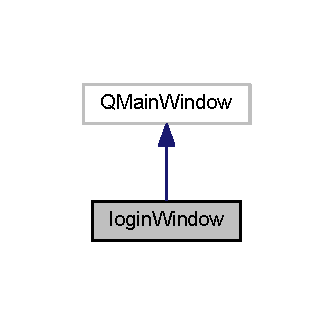
\includegraphics[width=160pt]{classlogin_window__inherit__graph}
\end{center}
\end{figure}


Collaboration diagram for login\+Window\+:\nopagebreak
\begin{figure}[H]
\begin{center}
\leavevmode
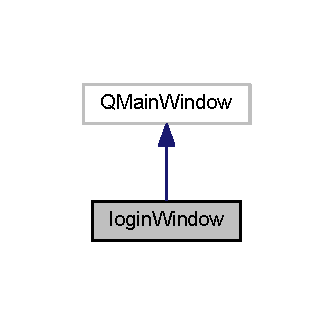
\includegraphics[width=160pt]{classlogin_window__coll__graph}
\end{center}
\end{figure}
\subsection*{Public Member Functions}
\begin{DoxyCompactItemize}
\item 
\hyperlink{classlogin_window_ad6f2de3f9d45e1f951a2eb2eeed9747e}{login\+Window} (Q\+Widget $\ast$parent=0)
\item 
Q\+String \hyperlink{classlogin_window_ae0670d5971676277b8d093e0396b4cb1}{get\+User\+Name\+Line\+Edit} ()
\end{DoxyCompactItemize}


\subsection{Detailed Description}

\begin{DoxyItemize}
\item 
\end{DoxyItemize}

\subsection{Constructor \& Destructor Documentation}
\mbox{\Hypertarget{classlogin_window_ad6f2de3f9d45e1f951a2eb2eeed9747e}\label{classlogin_window_ad6f2de3f9d45e1f951a2eb2eeed9747e}} 
\index{login\+Window@{login\+Window}!login\+Window@{login\+Window}}
\index{login\+Window@{login\+Window}!login\+Window@{login\+Window}}
\subsubsection{\texorpdfstring{login\+Window()}{loginWindow()}}
{\footnotesize\ttfamily login\+Window\+::login\+Window (\begin{DoxyParamCaption}\item[{Q\+Widget $\ast$}]{parent = {\ttfamily 0} }\end{DoxyParamCaption})\hspace{0.3cm}{\ttfamily [explicit]}}


\begin{DoxyItemize}
\item 
\begin{DoxyParams}{Parameters}
{\em parent} & \\
\hline
{\em parent} & \\
\hline
\end{DoxyParams}

\end{DoxyItemize}

\subsection{Member Function Documentation}
\mbox{\Hypertarget{classlogin_window_ae0670d5971676277b8d093e0396b4cb1}\label{classlogin_window_ae0670d5971676277b8d093e0396b4cb1}} 
\index{login\+Window@{login\+Window}!get\+User\+Name\+Line\+Edit@{get\+User\+Name\+Line\+Edit}}
\index{get\+User\+Name\+Line\+Edit@{get\+User\+Name\+Line\+Edit}!login\+Window@{login\+Window}}
\subsubsection{\texorpdfstring{get\+User\+Name\+Line\+Edit()}{getUserNameLineEdit()}}
{\footnotesize\ttfamily Q\+String login\+Window\+::get\+User\+Name\+Line\+Edit (\begin{DoxyParamCaption}{ }\end{DoxyParamCaption})}

fn get\+User\+Name\+Line\+Edit \begin{DoxyReturn}{Returns}

\end{DoxyReturn}


The documentation for this class was generated from the following files\+:\begin{DoxyCompactItemize}
\item 
loginwindow.\+h\item 
loginwindow.\+cpp\end{DoxyCompactItemize}

\hypertarget{class_ui_1_1_main_window}{}\section{Ui\+:\+:Main\+Window Class Reference}
\label{class_ui_1_1_main_window}\index{Ui\+::\+Main\+Window@{Ui\+::\+Main\+Window}}


Inheritance diagram for Ui\+:\+:Main\+Window\+:\nopagebreak
\begin{figure}[H]
\begin{center}
\leavevmode
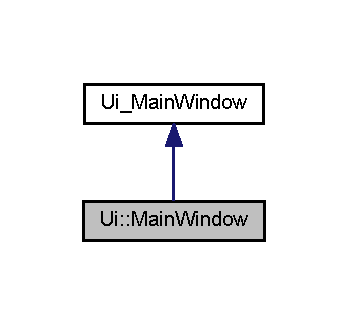
\includegraphics[width=167pt]{class_ui_1_1_main_window__inherit__graph}
\end{center}
\end{figure}


Collaboration diagram for Ui\+:\+:Main\+Window\+:\nopagebreak
\begin{figure}[H]
\begin{center}
\leavevmode
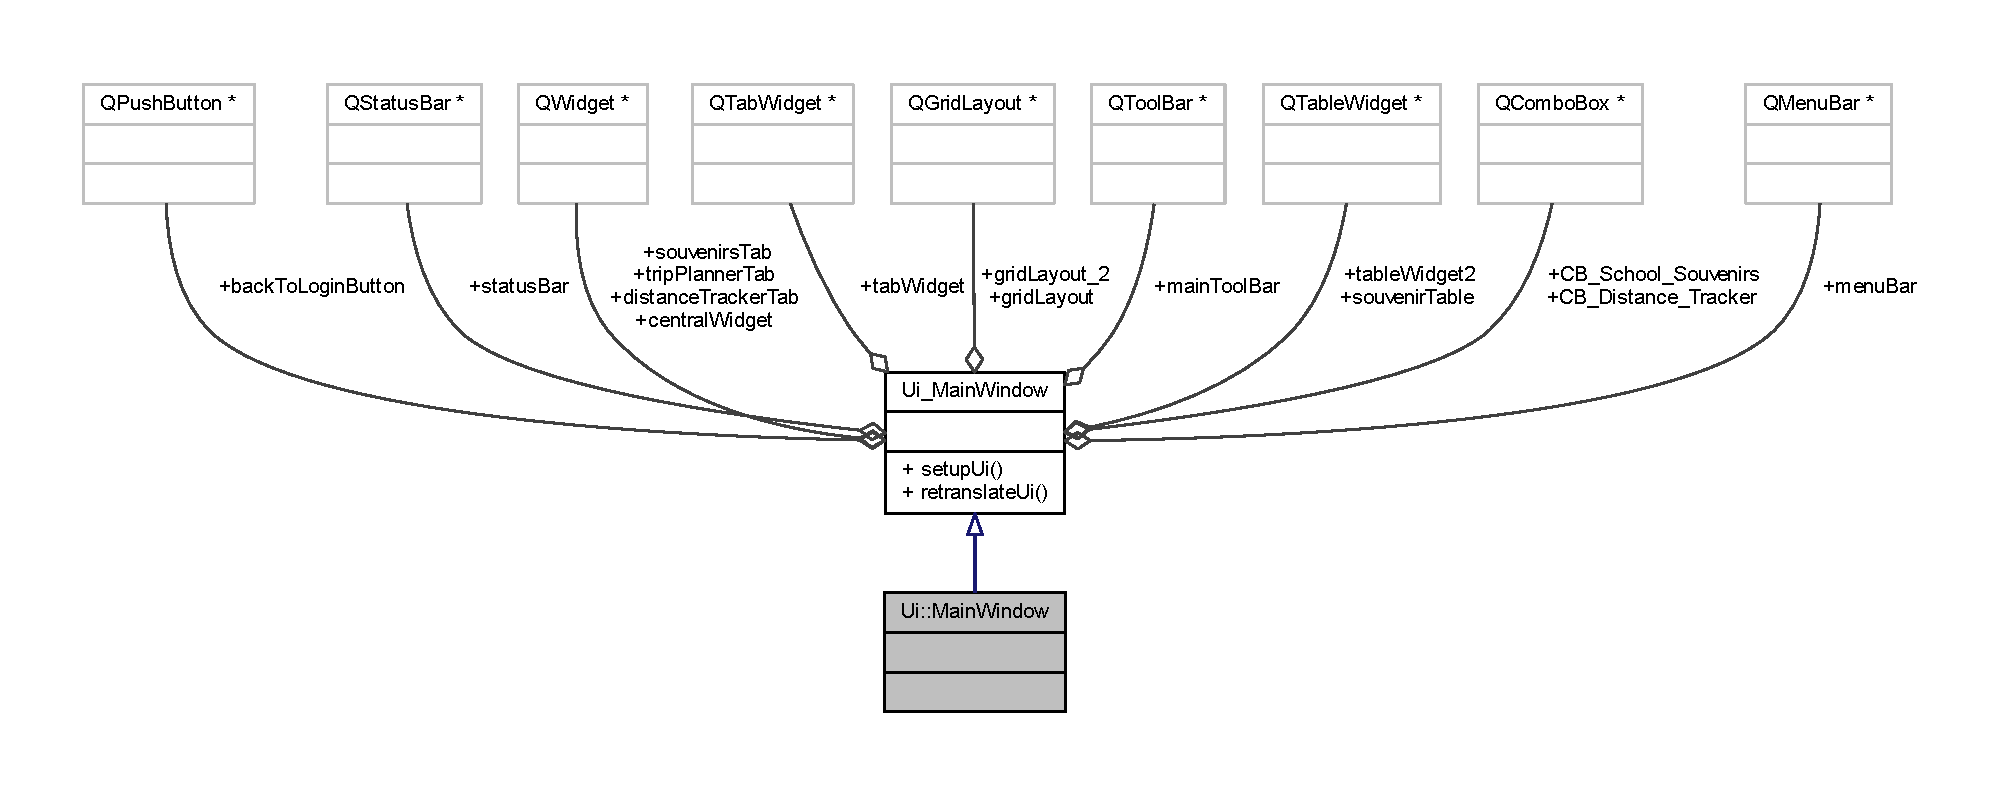
\includegraphics[width=167pt]{class_ui_1_1_main_window__coll__graph}
\end{center}
\end{figure}
\subsection*{Additional Inherited Members}


The documentation for this class was generated from the following file\+:\begin{DoxyCompactItemize}
\item 
ui\+\_\+mainwindow.\+h\end{DoxyCompactItemize}

\hypertarget{class_main_window}{}\section{Main\+Window Class Reference}
\label{class_main_window}\index{Main\+Window@{Main\+Window}}


Inheritance diagram for Main\+Window\+:\nopagebreak
\begin{figure}[H]
\begin{center}
\leavevmode
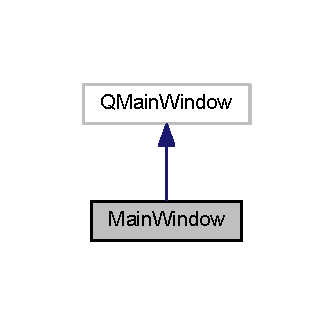
\includegraphics[width=173pt]{class_main_window__inherit__graph}
\end{center}
\end{figure}


Collaboration diagram for Main\+Window\+:\nopagebreak
\begin{figure}[H]
\begin{center}
\leavevmode
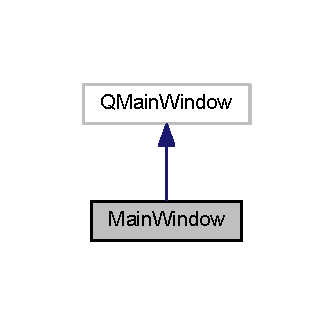
\includegraphics[width=173pt]{class_main_window__coll__graph}
\end{center}
\end{figure}
\subsection*{Public Member Functions}
\begin{DoxyCompactItemize}
\item 
\hyperlink{class_main_window_a8b244be8b7b7db1b08de2a2acb9409db}{Main\+Window} (Q\+Widget $\ast$parent=0)
\end{DoxyCompactItemize}


\subsection{Constructor \& Destructor Documentation}
\mbox{\Hypertarget{class_main_window_a8b244be8b7b7db1b08de2a2acb9409db}\label{class_main_window_a8b244be8b7b7db1b08de2a2acb9409db}} 
\index{Main\+Window@{Main\+Window}!Main\+Window@{Main\+Window}}
\index{Main\+Window@{Main\+Window}!Main\+Window@{Main\+Window}}
\subsubsection{\texorpdfstring{Main\+Window()}{MainWindow()}}
{\footnotesize\ttfamily Main\+Window\+::\+Main\+Window (\begin{DoxyParamCaption}\item[{Q\+Widget $\ast$}]{parent = {\ttfamily 0} }\end{DoxyParamCaption})\hspace{0.3cm}{\ttfamily [explicit]}}


\begin{DoxyParams}{Parameters}
{\em parent} & \\
\hline
\end{DoxyParams}
labels This sets up the Distance table in the user window

labels2 This sets up the souvenir table in the user window

DB This populates the drop down boxes for each user window 

The documentation for this class was generated from the following files\+:\begin{DoxyCompactItemize}
\item 
mainwindow.\+h\item 
mainwindow.\+cpp\end{DoxyCompactItemize}

\hypertarget{class_q_main_window}{}\section{Q\+Main\+Window Class Reference}
\label{class_q_main_window}\index{Q\+Main\+Window@{Q\+Main\+Window}}


Inheritance diagram for Q\+Main\+Window\+:\nopagebreak
\begin{figure}[H]
\begin{center}
\leavevmode
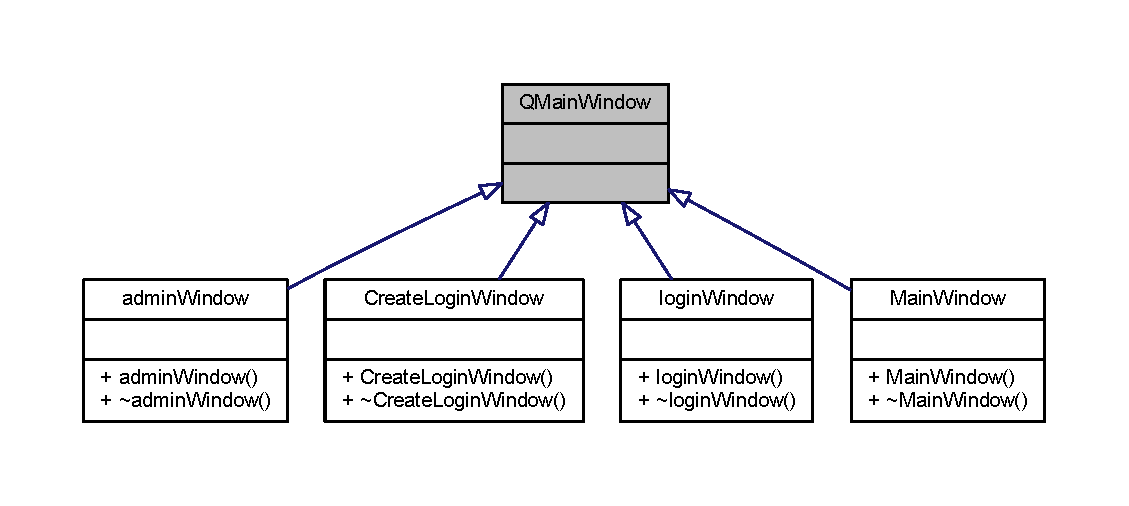
\includegraphics[width=350pt]{class_q_main_window__inherit__graph}
\end{center}
\end{figure}


Collaboration diagram for Q\+Main\+Window\+:\nopagebreak
\begin{figure}[H]
\begin{center}
\leavevmode
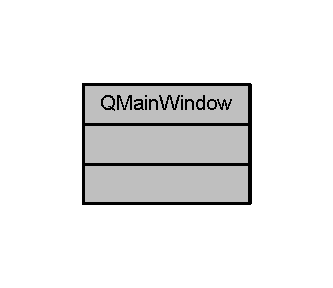
\includegraphics[width=160pt]{class_q_main_window__coll__graph}
\end{center}
\end{figure}


The documentation for this class was generated from the following file\+:\begin{DoxyCompactItemize}
\item 
mainwindow.\+h\end{DoxyCompactItemize}

\hypertarget{class_q_sql_database}{}\section{Q\+Sql\+Database Class Reference}
\label{class_q_sql_database}\index{Q\+Sql\+Database@{Q\+Sql\+Database}}


Inheritance diagram for Q\+Sql\+Database\+:\nopagebreak
\begin{figure}[H]
\begin{center}
\leavevmode
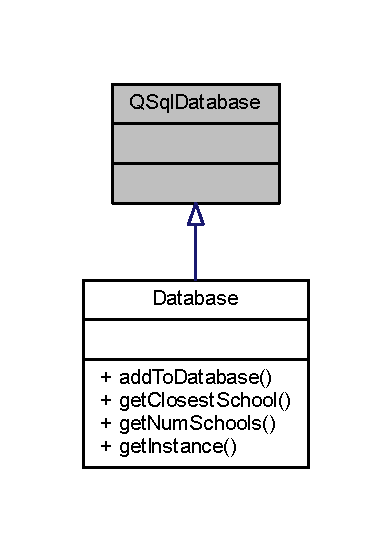
\includegraphics[width=188pt]{class_q_sql_database__inherit__graph}
\end{center}
\end{figure}


Collaboration diagram for Q\+Sql\+Database\+:\nopagebreak
\begin{figure}[H]
\begin{center}
\leavevmode
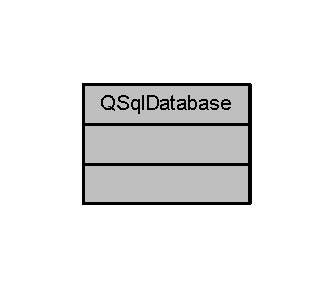
\includegraphics[width=160pt]{class_q_sql_database__coll__graph}
\end{center}
\end{figure}


The documentation for this class was generated from the following file\+:\begin{DoxyCompactItemize}
\item 
database.\+h\end{DoxyCompactItemize}

\hypertarget{classsouvenir}{}\section{souvenir Class Reference}
\label{classsouvenir}\index{souvenir@{souvenir}}


Collaboration diagram for souvenir\+:\nopagebreak
\begin{figure}[H]
\begin{center}
\leavevmode
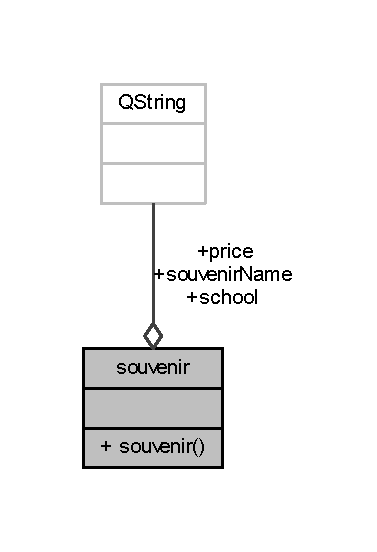
\includegraphics[width=181pt]{classsouvenir__coll__graph}
\end{center}
\end{figure}
\subsection*{Public Member Functions}
\begin{DoxyCompactItemize}
\item 
\hyperlink{classsouvenir_a53eb7933555c5ba83d336c5b21475cc2}{souvenir} (Q\+String school\+Name, Q\+String souvenir\+Name, Q\+String price)
\end{DoxyCompactItemize}
\subsection*{Public Attributes}
\begin{DoxyCompactItemize}
\item 
\mbox{\Hypertarget{classsouvenir_a5c5db004874f514b60fba59b3a6e8d2d}\label{classsouvenir_a5c5db004874f514b60fba59b3a6e8d2d}} 
Q\+String {\bfseries school}
\item 
\mbox{\Hypertarget{classsouvenir_af5e9cd9f582373994b70065f64160a97}\label{classsouvenir_af5e9cd9f582373994b70065f64160a97}} 
Q\+String {\bfseries souvenir\+Name}
\item 
\mbox{\Hypertarget{classsouvenir_a79e0d7bf9536730792ad23f3f2a0f791}\label{classsouvenir_a79e0d7bf9536730792ad23f3f2a0f791}} 
Q\+String {\bfseries price}
\end{DoxyCompactItemize}


\subsection{Constructor \& Destructor Documentation}
\mbox{\Hypertarget{classsouvenir_a53eb7933555c5ba83d336c5b21475cc2}\label{classsouvenir_a53eb7933555c5ba83d336c5b21475cc2}} 
\index{souvenir@{souvenir}!souvenir@{souvenir}}
\index{souvenir@{souvenir}!souvenir@{souvenir}}
\subsubsection{\texorpdfstring{souvenir()}{souvenir()}}
{\footnotesize\ttfamily souvenir\+::souvenir (\begin{DoxyParamCaption}\item[{Q\+String}]{school\+Name,  }\item[{Q\+String}]{souvenir\+Name,  }\item[{Q\+String}]{price }\end{DoxyParamCaption})\hspace{0.3cm}{\ttfamily [inline]}}


\begin{DoxyParams}{Parameters}
{\em school\+Name} & \\
\hline
{\em souvenir\+Name} & \\
\hline
{\em price} & \\
\hline
\end{DoxyParams}


The documentation for this class was generated from the following file\+:\begin{DoxyCompactItemize}
\item 
souvenir.\+h\end{DoxyCompactItemize}

\hypertarget{class_the}{}\section{The Class Reference}
\label{class_the}\index{The@{The}}


Collaboration diagram for The\+:\nopagebreak
\begin{figure}[H]
\begin{center}
\leavevmode
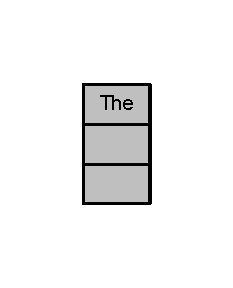
\includegraphics[width=112pt]{class_the__coll__graph}
\end{center}
\end{figure}


\subsection{Detailed Description}

\begin{DoxyItemize}
\item 
\end{DoxyItemize}

The documentation for this class was generated from the following file\+:\begin{DoxyCompactItemize}
\item 
mainwindow.\+h\end{DoxyCompactItemize}

\hypertarget{class_ui___main_window}{}\section{Ui\+\_\+\+Main\+Window Class Reference}
\label{class_ui___main_window}\index{Ui\+\_\+\+Main\+Window@{Ui\+\_\+\+Main\+Window}}


Inheritance diagram for Ui\+\_\+\+Main\+Window\+:\nopagebreak
\begin{figure}[H]
\begin{center}
\leavevmode
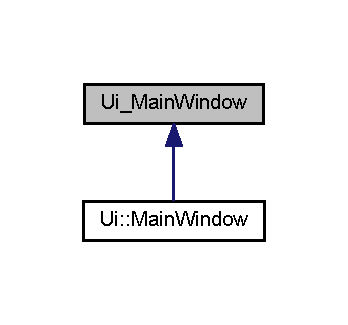
\includegraphics[width=167pt]{class_ui___main_window__inherit__graph}
\end{center}
\end{figure}
\subsection*{Public Member Functions}
\begin{DoxyCompactItemize}
\item 
\mbox{\Hypertarget{class_ui___main_window_acf4a0872c4c77d8f43a2ec66ed849b58}\label{class_ui___main_window_acf4a0872c4c77d8f43a2ec66ed849b58}} 
void {\bfseries setup\+Ui} (Q\+Main\+Window $\ast$\hyperlink{class_main_window}{Main\+Window})
\item 
\mbox{\Hypertarget{class_ui___main_window_a097dd160c3534a204904cb374412c618}\label{class_ui___main_window_a097dd160c3534a204904cb374412c618}} 
void {\bfseries retranslate\+Ui} (Q\+Main\+Window $\ast$\hyperlink{class_main_window}{Main\+Window})
\end{DoxyCompactItemize}
\subsection*{Public Attributes}
\begin{DoxyCompactItemize}
\item 
\mbox{\Hypertarget{class_ui___main_window_a30075506c2116c3ed4ff25e07ae75f81}\label{class_ui___main_window_a30075506c2116c3ed4ff25e07ae75f81}} 
Q\+Widget $\ast$ {\bfseries central\+Widget}
\item 
\mbox{\Hypertarget{class_ui___main_window_a6b2a0c5f7e8ff2a87134908dd770d2d2}\label{class_ui___main_window_a6b2a0c5f7e8ff2a87134908dd770d2d2}} 
Q\+Grid\+Layout $\ast$ {\bfseries grid\+Layout\+\_\+2}
\item 
\mbox{\Hypertarget{class_ui___main_window_aecd96a04789fcfec3f98d80390ad8184}\label{class_ui___main_window_aecd96a04789fcfec3f98d80390ad8184}} 
Q\+V\+Box\+Layout $\ast$ {\bfseries vertical\+Layout}
\item 
\mbox{\Hypertarget{class_ui___main_window_a3260b943854b841c986f47c4726ee7f9}\label{class_ui___main_window_a3260b943854b841c986f47c4726ee7f9}} 
Q\+Tab\+Widget $\ast$ {\bfseries tab\+Widget}
\item 
\mbox{\Hypertarget{class_ui___main_window_a89c881d7aacd60aca9053c00cb8d5c20}\label{class_ui___main_window_a89c881d7aacd60aca9053c00cb8d5c20}} 
Q\+Widget $\ast$ {\bfseries trip\+Planner\+Tab}
\item 
\mbox{\Hypertarget{class_ui___main_window_a6fd1d1c1e8ea725340e6088dda793551}\label{class_ui___main_window_a6fd1d1c1e8ea725340e6088dda793551}} 
Q\+Label $\ast$ {\bfseries Us\+\_\+pixelmap}
\item 
\mbox{\Hypertarget{class_ui___main_window_a212706d1b737fef1e79ae00b6a9d072c}\label{class_ui___main_window_a212706d1b737fef1e79ae00b6a9d072c}} 
Q\+Text\+Browser $\ast$ {\bfseries test\+Browser}
\item 
\mbox{\Hypertarget{class_ui___main_window_a580c648c54335179505ae6394063ff9f}\label{class_ui___main_window_a580c648c54335179505ae6394063ff9f}} 
Q\+Push\+Button $\ast$ {\bfseries Saddleback\+Button}
\item 
\mbox{\Hypertarget{class_ui___main_window_a08bc10609d1d246d840b64cd8a3d4c5f}\label{class_ui___main_window_a08bc10609d1d246d840b64cd8a3d4c5f}} 
Q\+Push\+Button $\ast$ {\bfseries U\+C\+I\+Button}
\item 
\mbox{\Hypertarget{class_ui___main_window_a351a3b2f3ffcf60eee58939b8899bbf5}\label{class_ui___main_window_a351a3b2f3ffcf60eee58939b8899bbf5}} 
Q\+Push\+Button $\ast$ {\bfseries U\+C\+L\+A\+Button}
\item 
\mbox{\Hypertarget{class_ui___main_window_aae679a28f5d6edb3052fdd1a4a58cba7}\label{class_ui___main_window_aae679a28f5d6edb3052fdd1a4a58cba7}} 
Q\+Check\+Box $\ast$ {\bfseries automatic\+Route\+Tracking\+Check\+Box}
\item 
\mbox{\Hypertarget{class_ui___main_window_a3043f9308a2bff128c4f6b6e90c797e5}\label{class_ui___main_window_a3043f9308a2bff128c4f6b6e90c797e5}} 
Q\+Label $\ast$ {\bfseries Total\+Miles\+Label}
\item 
\mbox{\Hypertarget{class_ui___main_window_a48a32a92d66ce272d5545a935fc52eac}\label{class_ui___main_window_a48a32a92d66ce272d5545a935fc52eac}} 
Q\+Push\+Button $\ast$ {\bfseries University\+Of\+Pacific\+Button}
\item 
\mbox{\Hypertarget{class_ui___main_window_aaba0b3ac63b7e8d2442b5946bc39d897}\label{class_ui___main_window_aaba0b3ac63b7e8d2442b5946bc39d897}} 
Q\+Push\+Button $\ast$ {\bfseries University\+Of\+Oregon\+Button}
\item 
\mbox{\Hypertarget{class_ui___main_window_ae9795c18b36e81c9850f01429924742a}\label{class_ui___main_window_ae9795c18b36e81c9850f01429924742a}} 
Q\+Push\+Button $\ast$ {\bfseries A\+S\+U\+Button}
\item 
\mbox{\Hypertarget{class_ui___main_window_a62af8ed4d24d92946db6767ede29ceba}\label{class_ui___main_window_a62af8ed4d24d92946db6767ede29ceba}} 
Q\+Push\+Button $\ast$ {\bfseries University\+Of\+Wisconsin\+Button}
\item 
\mbox{\Hypertarget{class_ui___main_window_ad67005e00d0006396589b4b4640387d0}\label{class_ui___main_window_ad67005e00d0006396589b4b4640387d0}} 
Q\+Push\+Button $\ast$ {\bfseries Northwestern\+Button}
\item 
\mbox{\Hypertarget{class_ui___main_window_ad707347705abc7de8fffbe394e2aafa6}\label{class_ui___main_window_ad707347705abc7de8fffbe394e2aafa6}} 
Q\+Push\+Button $\ast$ {\bfseries University\+Of\+Michigan\+Button}
\item 
\mbox{\Hypertarget{class_ui___main_window_aee1dc89fbeaf7196d6e12136b8f78c1b}\label{class_ui___main_window_aee1dc89fbeaf7196d6e12136b8f78c1b}} 
Q\+Push\+Button $\ast$ {\bfseries O\+S\+U\+Button}
\item 
\mbox{\Hypertarget{class_ui___main_window_aff9c6037c833031dc66349edba8ff2ee}\label{class_ui___main_window_aff9c6037c833031dc66349edba8ff2ee}} 
Q\+Push\+Button $\ast$ {\bfseries M\+I\+T\+Button}
\item 
\mbox{\Hypertarget{class_ui___main_window_a62ac72ca9e1a0c9d85e06da70742313e}\label{class_ui___main_window_a62ac72ca9e1a0c9d85e06da70742313e}} 
Q\+Push\+Button $\ast$ {\bfseries key\+Button}
\item 
\mbox{\Hypertarget{class_ui___main_window_a29c330db2deecc10de9607628a8664d1}\label{class_ui___main_window_a29c330db2deecc10de9607628a8664d1}} 
Q\+Push\+Button $\ast$ {\bfseries Fullerton\+Button}
\item 
\mbox{\Hypertarget{class_ui___main_window_a2f715dc39f1ea1ddc9ed415fb3e9196c}\label{class_ui___main_window_a2f715dc39f1ea1ddc9ed415fb3e9196c}} 
Q\+Push\+Button $\ast$ {\bfseries Texas\+Button}
\item 
\mbox{\Hypertarget{class_ui___main_window_a63d698a8afb3781e9b02408426f39eb8}\label{class_ui___main_window_a63d698a8afb3781e9b02408426f39eb8}} 
Q\+Spin\+Box $\ast$ {\bfseries num\+Of\+Schools\+Wheel}
\item 
\mbox{\Hypertarget{class_ui___main_window_a9a1d6d24bba2c52c06d10805b6456d13}\label{class_ui___main_window_a9a1d6d24bba2c52c06d10805b6456d13}} 
Q\+Label $\ast$ {\bfseries num\+Of\+Schools\+To\+Visit\+Label}
\item 
\mbox{\Hypertarget{class_ui___main_window_a2ebb4530ef6c8b3fc3147c401cc8df6e}\label{class_ui___main_window_a2ebb4530ef6c8b3fc3147c401cc8df6e}} 
Q\+Push\+Button $\ast$ {\bfseries remove\+Prev\+Des\+Button}
\item 
\mbox{\Hypertarget{class_ui___main_window_a9c2647e3ca1e759d9bfa1ff21e6acb1f}\label{class_ui___main_window_a9c2647e3ca1e759d9bfa1ff21e6acb1f}} 
Q\+Widget $\ast$ {\bfseries distance\+Tracker\+Tab}
\item 
\mbox{\Hypertarget{class_ui___main_window_a22d4df181bec9dfed94facfe029c76f0}\label{class_ui___main_window_a22d4df181bec9dfed94facfe029c76f0}} 
Q\+Combo\+Box $\ast$ {\bfseries C\+B\+\_\+\+Distance\+\_\+\+Tracker}
\item 
\mbox{\Hypertarget{class_ui___main_window_a2265350de498058d76a442c5446ca0dd}\label{class_ui___main_window_a2265350de498058d76a442c5446ca0dd}} 
Q\+Table\+Widget $\ast$ {\bfseries table\+Widget2}
\item 
\mbox{\Hypertarget{class_ui___main_window_a61af9bb6c545f530d061e2b1a4e9d6f9}\label{class_ui___main_window_a61af9bb6c545f530d061e2b1a4e9d6f9}} 
Q\+Widget $\ast$ {\bfseries souvenirs\+Tab}
\item 
\mbox{\Hypertarget{class_ui___main_window_a424c42420628072eea73d3472abd4836}\label{class_ui___main_window_a424c42420628072eea73d3472abd4836}} 
Q\+Combo\+Box $\ast$ {\bfseries C\+B\+\_\+\+School\+\_\+\+Souvenirs}
\item 
\mbox{\Hypertarget{class_ui___main_window_a5ba338b74df905a52cff88d140783226}\label{class_ui___main_window_a5ba338b74df905a52cff88d140783226}} 
Q\+Table\+Widget $\ast$ {\bfseries souvenir\+Table}
\item 
\mbox{\Hypertarget{class_ui___main_window_a3efc28c664e9f5115095aafbbc5ac6bc}\label{class_ui___main_window_a3efc28c664e9f5115095aafbbc5ac6bc}} 
Q\+Widget $\ast$ {\bfseries tab}
\item 
\mbox{\Hypertarget{class_ui___main_window_ad9c89133780f28e6efa2ec17ceb9cff5}\label{class_ui___main_window_ad9c89133780f28e6efa2ec17ceb9cff5}} 
Q\+Label $\ast$ {\bfseries label}
\item 
\mbox{\Hypertarget{class_ui___main_window_a23c8aadca0eed43ef89d19aa17503981}\label{class_ui___main_window_a23c8aadca0eed43ef89d19aa17503981}} 
Q\+Text\+Browser $\ast$ {\bfseries help\+Text\+Browser}
\item 
\mbox{\Hypertarget{class_ui___main_window_aa5800f4d4be2cfb760f58ef468c53a1a}\label{class_ui___main_window_aa5800f4d4be2cfb760f58ef468c53a1a}} 
Q\+Push\+Button $\ast$ {\bfseries back\+To\+Login\+Button}
\item 
\mbox{\Hypertarget{class_ui___main_window_a2be1c24ec9adfca18e1dcc951931457f}\label{class_ui___main_window_a2be1c24ec9adfca18e1dcc951931457f}} 
Q\+Menu\+Bar $\ast$ {\bfseries menu\+Bar}
\item 
\mbox{\Hypertarget{class_ui___main_window_a50fa481337604bcc8bf68de18ab16ecd}\label{class_ui___main_window_a50fa481337604bcc8bf68de18ab16ecd}} 
Q\+Status\+Bar $\ast$ {\bfseries status\+Bar}
\end{DoxyCompactItemize}


The documentation for this class was generated from the following file\+:\begin{DoxyCompactItemize}
\item 
ui\+\_\+mainwindow.\+h\end{DoxyCompactItemize}

\hypertarget{classwindow_holder}{}\section{window\+Holder Class Reference}
\label{classwindow_holder}\index{window\+Holder@{window\+Holder}}
\subsection*{Public Member Functions}
\begin{DoxyCompactItemize}
\item 
\mbox{\Hypertarget{classwindow_holder_ab49515f6a1641726cc90cfe25c590dc9}\label{classwindow_holder_ab49515f6a1641726cc90cfe25c590dc9}} 
void {\bfseries Main\+Window\+Hide} ()
\item 
\mbox{\Hypertarget{classwindow_holder_a896305f2187010582bec985c69732f50}\label{classwindow_holder_a896305f2187010582bec985c69732f50}} 
void {\bfseries Main\+Window\+Show} ()
\item 
\mbox{\Hypertarget{classwindow_holder_ab8a34349cac278a51b2bbf58c32d2c8c}\label{classwindow_holder_ab8a34349cac278a51b2bbf58c32d2c8c}} 
void {\bfseries Login\+Window\+Hide} ()
\item 
\mbox{\Hypertarget{classwindow_holder_ad360d5183c9b9121ee3533f55228cafe}\label{classwindow_holder_ad360d5183c9b9121ee3533f55228cafe}} 
void {\bfseries Login\+Window\+Show} ()
\item 
\mbox{\Hypertarget{classwindow_holder_aa459aa3bd4a409b838ea2c0b1be67f37}\label{classwindow_holder_aa459aa3bd4a409b838ea2c0b1be67f37}} 
void {\bfseries Admin\+Window\+Hide} ()
\item 
\mbox{\Hypertarget{classwindow_holder_a0c97d703dc433ee2e20b89efa849780c}\label{classwindow_holder_a0c97d703dc433ee2e20b89efa849780c}} 
void {\bfseries Admin\+Window\+Show} ()
\item 
\mbox{\Hypertarget{classwindow_holder_a816f65a254c2636fa7221d401809bcc0}\label{classwindow_holder_a816f65a254c2636fa7221d401809bcc0}} 
void {\bfseries Create\+Window\+Hide} ()
\item 
\mbox{\Hypertarget{classwindow_holder_af35553dd4cd1f109ce3b72835e3d7180}\label{classwindow_holder_af35553dd4cd1f109ce3b72835e3d7180}} 
void {\bfseries Create\+Window\+Show} ()
\item 
\mbox{\Hypertarget{classwindow_holder_ad1027581c042b76dea11b819da81b834}\label{classwindow_holder_ad1027581c042b76dea11b819da81b834}} 
void {\bfseries key\+Window\+Hide} ()
\item 
\mbox{\Hypertarget{classwindow_holder_a8492fcdd5346b1b437b5c2671c26ac98}\label{classwindow_holder_a8492fcdd5346b1b437b5c2671c26ac98}} 
void {\bfseries key\+Window\+Show} ()
\item 
\mbox{\Hypertarget{classwindow_holder_af2ed7a4ab1231e76da3c757eb1e71423}\label{classwindow_holder_af2ed7a4ab1231e76da3c757eb1e71423}} 
void {\bfseries shopping\+Window\+Hide} ()
\item 
\mbox{\Hypertarget{classwindow_holder_aba9de893b828fdd8efdc13e453608948}\label{classwindow_holder_aba9de893b828fdd8efdc13e453608948}} 
void {\bfseries shopping\+Window\+Show} ()
\item 
void \hyperlink{classwindow_holder_ab51ad6c3e9cdfd245729fe59958e00ce}{set\+Shop\+Button} (Q\+String school)
\item 
\mbox{\Hypertarget{classwindow_holder_aae2ea03e3a26645b07076b3b23a3f8e2}\label{classwindow_holder_aae2ea03e3a26645b07076b3b23a3f8e2}} 
void {\bfseries show\+Shop\+Next\+School\+Button} ()
\item 
\mbox{\Hypertarget{classwindow_holder_a5315d6fbe8abbc60f9821aebeb9c6680}\label{classwindow_holder_a5315d6fbe8abbc60f9821aebeb9c6680}} 
void {\bfseries hide\+Shop\+Next\+School\+Button} ()
\item 
\mbox{\Hypertarget{classwindow_holder_a4f3d4ae38674aa668e782d2c98d0e325}\label{classwindow_holder_a4f3d4ae38674aa668e782d2c98d0e325}} 
void {\bfseries main\+Update\+UI} ()
\item 
\mbox{\Hypertarget{classwindow_holder_ade6b40649d85b1188d1a12ce3f76b7f7}\label{classwindow_holder_ade6b40649d85b1188d1a12ce3f76b7f7}} 
void {\bfseries main\+Inc\+Index} ()
\item 
\mbox{\Hypertarget{classwindow_holder_ab4bf93b4741176fe4fb38465278227ad}\label{classwindow_holder_ab4bf93b4741176fe4fb38465278227ad}} 
void {\bfseries update\+Shop\+Window} ()
\item 
\mbox{\Hypertarget{classwindow_holder_abbd6d065957630393a4337acd493070b}\label{classwindow_holder_abbd6d065957630393a4337acd493070b}} 
void {\bfseries checkout\+Window\+Hide} ()
\item 
\mbox{\Hypertarget{classwindow_holder_ab302a5831c4e9c65329f3b13afd15911}\label{classwindow_holder_ab302a5831c4e9c65329f3b13afd15911}} 
void {\bfseries checkout\+Window\+Show} ()
\item 
Q\+String \hyperlink{classwindow_holder_a2acbd88adbc48d8e9aef05ce5a692239}{get\+User\+Name} ()
\item 
\mbox{\Hypertarget{classwindow_holder_a7c7365b2c6cc19052ef677e383c021a3}\label{classwindow_holder_a7c7365b2c6cc19052ef677e383c021a3}} 
void {\bfseries set\+Main\+Username} ()
\item 
Q\+String \hyperlink{classwindow_holder_ad152c410bf87d7a04f4fde66253685c2}{get\+Username} ()
\item 
\mbox{\Hypertarget{classwindow_holder_acff6a10c006a734343dfb67ec6b78249}\label{classwindow_holder_acff6a10c006a734343dfb67ec6b78249}} 
void {\bfseries clear\+Shopping\+Cart} ()
\end{DoxyCompactItemize}
\subsection*{Static Public Member Functions}
\begin{DoxyCompactItemize}
\item 
static \hyperlink{classwindow_holder}{window\+Holder} $\ast$ \hyperlink{classwindow_holder_ae64d5ca66adacd67952c0d4d45dc6409}{get\+Instance} ()
\end{DoxyCompactItemize}


\subsection{Member Function Documentation}
\mbox{\Hypertarget{classwindow_holder_ae64d5ca66adacd67952c0d4d45dc6409}\label{classwindow_holder_ae64d5ca66adacd67952c0d4d45dc6409}} 
\index{window\+Holder@{window\+Holder}!get\+Instance@{get\+Instance}}
\index{get\+Instance@{get\+Instance}!window\+Holder@{window\+Holder}}
\subsubsection{\texorpdfstring{get\+Instance()}{getInstance()}}
{\footnotesize\ttfamily \hyperlink{classwindow_holder}{window\+Holder} $\ast$ window\+Holder\+::get\+Instance (\begin{DoxyParamCaption}{ }\end{DoxyParamCaption})\hspace{0.3cm}{\ttfamily [static]}}

\begin{DoxyReturn}{Returns}

\end{DoxyReturn}
if the instance is still a nullptr

create a new instance

if the instance exists, it\textquotesingle{}ll return a copy of the isntance \mbox{\Hypertarget{classwindow_holder_a2acbd88adbc48d8e9aef05ce5a692239}\label{classwindow_holder_a2acbd88adbc48d8e9aef05ce5a692239}} 
\index{window\+Holder@{window\+Holder}!get\+User\+Name@{get\+User\+Name}}
\index{get\+User\+Name@{get\+User\+Name}!window\+Holder@{window\+Holder}}
\subsubsection{\texorpdfstring{get\+User\+Name()}{getUserName()}}
{\footnotesize\ttfamily window\+Holder\+::get\+User\+Name (\begin{DoxyParamCaption}{ }\end{DoxyParamCaption})\hspace{0.3cm}{\ttfamily [inline]}}

\begin{DoxyReturn}{Returns}

\end{DoxyReturn}
\mbox{\Hypertarget{classwindow_holder_ad152c410bf87d7a04f4fde66253685c2}\label{classwindow_holder_ad152c410bf87d7a04f4fde66253685c2}} 
\index{window\+Holder@{window\+Holder}!get\+Username@{get\+Username}}
\index{get\+Username@{get\+Username}!window\+Holder@{window\+Holder}}
\subsubsection{\texorpdfstring{get\+Username()}{getUsername()}}
{\footnotesize\ttfamily window\+Holder\+::get\+Username (\begin{DoxyParamCaption}{ }\end{DoxyParamCaption})\hspace{0.3cm}{\ttfamily [inline]}}

\begin{DoxyReturn}{Returns}

\end{DoxyReturn}
\mbox{\Hypertarget{classwindow_holder_ab51ad6c3e9cdfd245729fe59958e00ce}\label{classwindow_holder_ab51ad6c3e9cdfd245729fe59958e00ce}} 
\index{window\+Holder@{window\+Holder}!set\+Shop\+Button@{set\+Shop\+Button}}
\index{set\+Shop\+Button@{set\+Shop\+Button}!window\+Holder@{window\+Holder}}
\subsubsection{\texorpdfstring{set\+Shop\+Button()}{setShopButton()}}
{\footnotesize\ttfamily window\+Holder\+::set\+Shop\+Button (\begin{DoxyParamCaption}\item[{Q\+String}]{school }\end{DoxyParamCaption})\hspace{0.3cm}{\ttfamily [inline]}}


\begin{DoxyParams}{Parameters}
{\em school} & \\
\hline
\end{DoxyParams}


The documentation for this class was generated from the following files\+:\begin{DoxyCompactItemize}
\item 
windowholder.\+h\item 
windowholder.\+cpp\end{DoxyCompactItemize}

%--- End generated contents ---

% Index
\backmatter
\newpage
\phantomsection
\clearemptydoublepage
\addcontentsline{toc}{chapter}{Index}
\printindex

\end{document}
